% \documentclass[aspectratio=169]{beamer} % 16:9
\documentclass{beamer}
\usepackage{ctex, hyperref}
\usepackage[T1]{fontenc}
\graphicspath{{pic/}}  % 定义图片路径
\usefonttheme[onlymath]{serif} % 改公式字体为衬线
% other packages
\usepackage{latexsym, amsmath, amsfonts, xcolor, multicol, booktabs, calligra}
\usepackage{graphicx, pstricks, listings, stackengine}

\author[Sunbowen Lee]{李孙博闻}
\title[Graph neural network]{图卷积神经网络温和入门}
% \subtitle{图神经网络介绍}
\institute{武汉科技大学 \\ 理学院 \\ 冶金工业过程系统科学湖北省重点实验室}
\date{\today}

\usepackage{wust}  % 使用WUST风格模板

\lstset{
    basicstyle=\ttfamily\small,
    keywordstyle=\bfseries\color{deepblue},
    emphstyle=\ttfamily\color{deepred},    % Custom highlighting style
    stringstyle=\color{deepgreen},
    numbers=left,
    numberstyle=\small\color{halfgray},
    rulesepcolor=\color{red!20!green!20!blue!20},
    frame=shadowbox,
}

\begin{document}

\songti % 字体
\setsansfont{Times New Roman} % 英文衬线

\begin{frame}  % 封面
    \titlepage
    \begin{figure}[htpb]
        \centering
        \vspace{-0.7cm}
        
\includegraphics[width=0.45\linewidth]{wust.png}
    \end{figure}
\end{frame}

\begin{frame}{前言}
    尽管图网络具体实现可通过简单调包实现, 但在此之前仍然需要了解图的基础知识, 特别是``图嵌入''和``信息传递''的概念. \newline

    本幻灯片材料主要参考Sanchez-Lengeling\cite{sanchez-lengeling2021a}等人的论文。
\end{frame}

\begin{frame}{目录}\small
    \tableofcontents[subsectionstyle=hide]
\end{frame}

\AtBeginSubsection[]{
    \begin{frame}
        \tableofcontents[currentsubsection]
    \end{frame}
}

\section{图结构基础}

% \begin{itemize} % [<+-| alert@+>]

\begin{frame}{Vertex, Edge and Global}
    \begin{figure}
        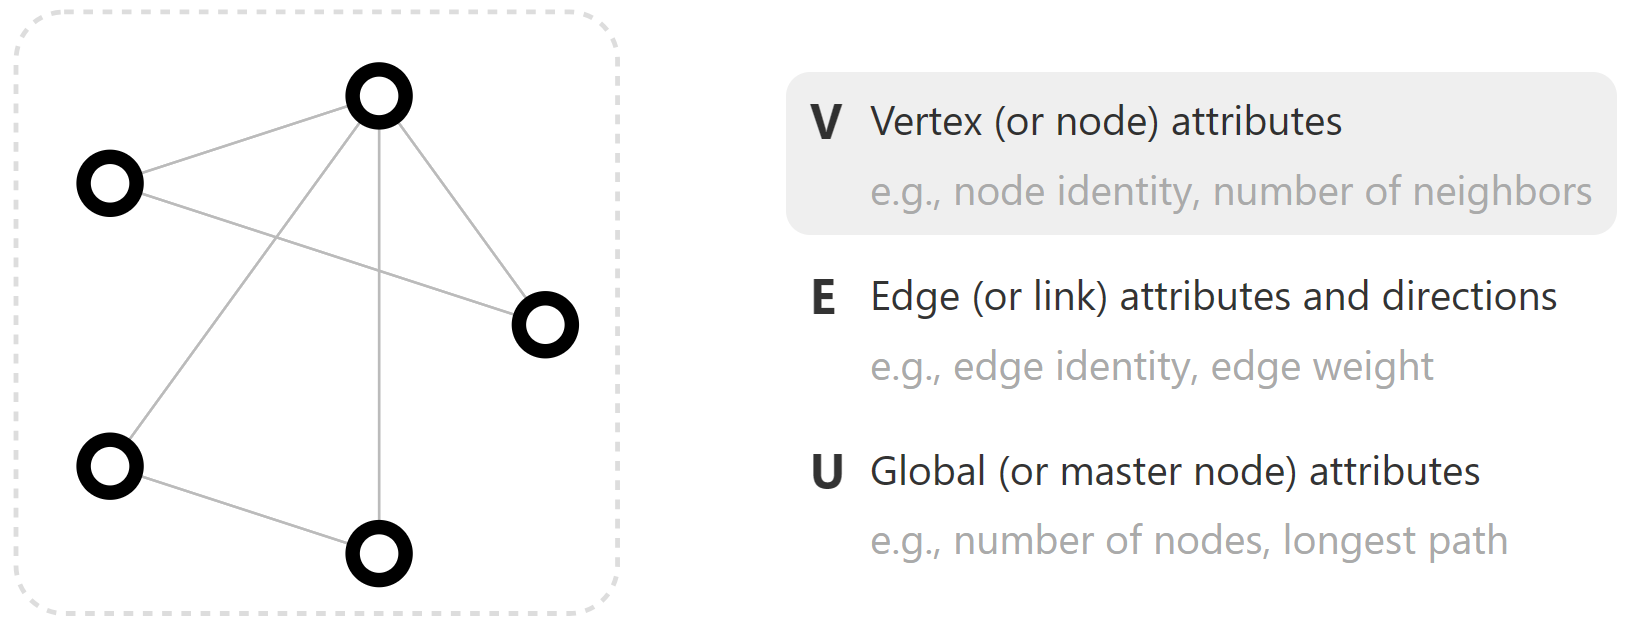
\includegraphics[width=\textwidth]{vertex.png}
        \caption{节点,节点一般有自己的特征。}
    \end{figure}
\end{frame}

\begin{frame}{Vertex, Edge and Global}
    \begin{figure}
        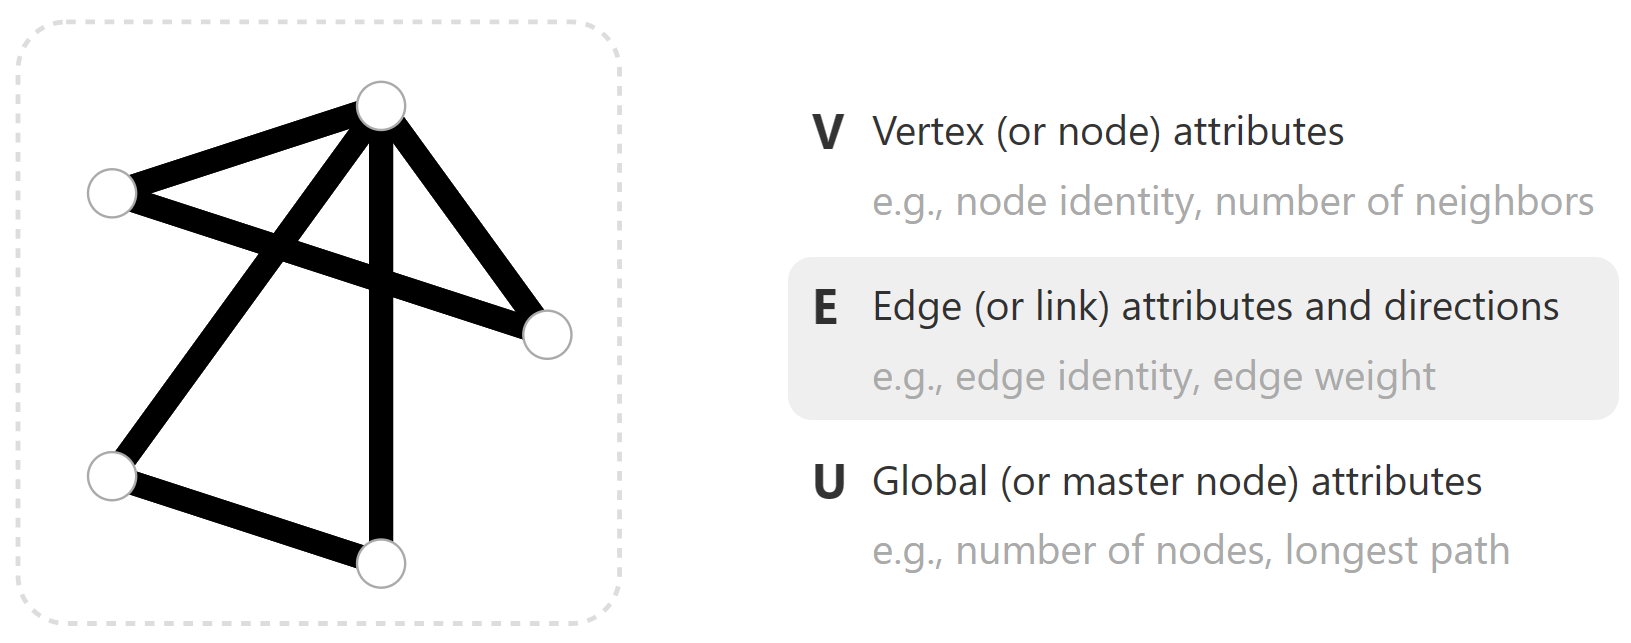
\includegraphics[width=\textwidth]{edge.png}
        \caption{边,节点一般也有自己的特征。}
    \end{figure}
\end{frame}

\begin{frame}{Vertex, Edge and Global}
    \begin{figure}
        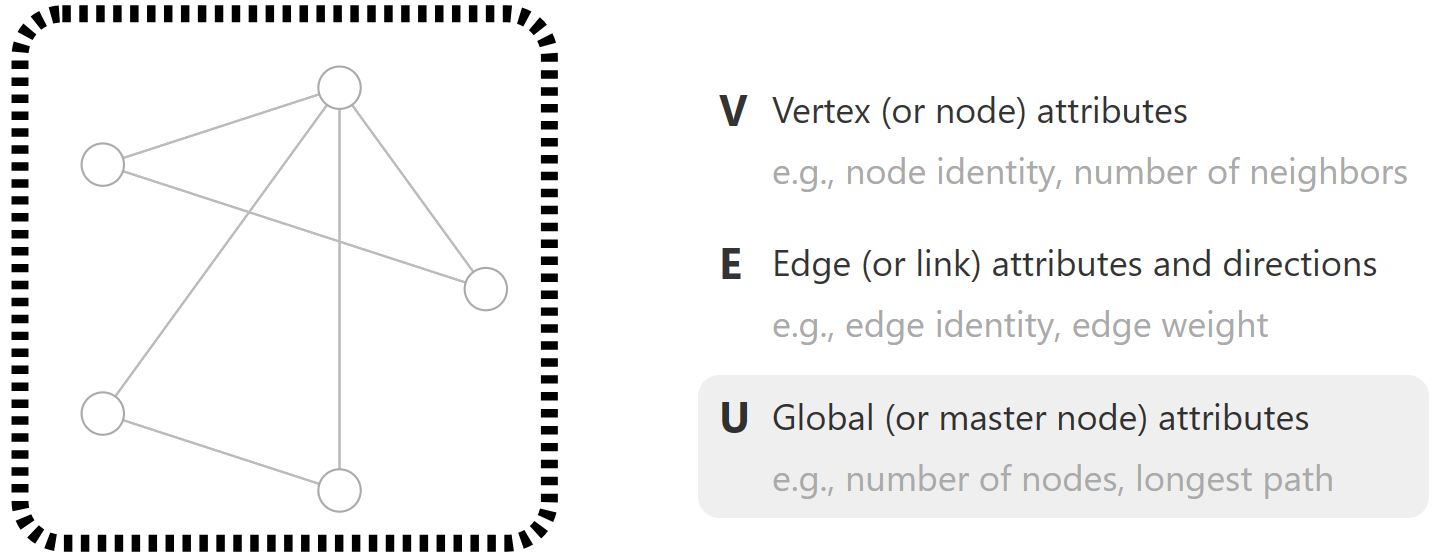
\includegraphics[width=\textwidth]{global.png}
        \caption{全局特征,做图分类任务的时候存在。}
    \end{figure}
\end{frame}

\begin{frame}{Vertex, Edge and Global}
    \begin{figure}
        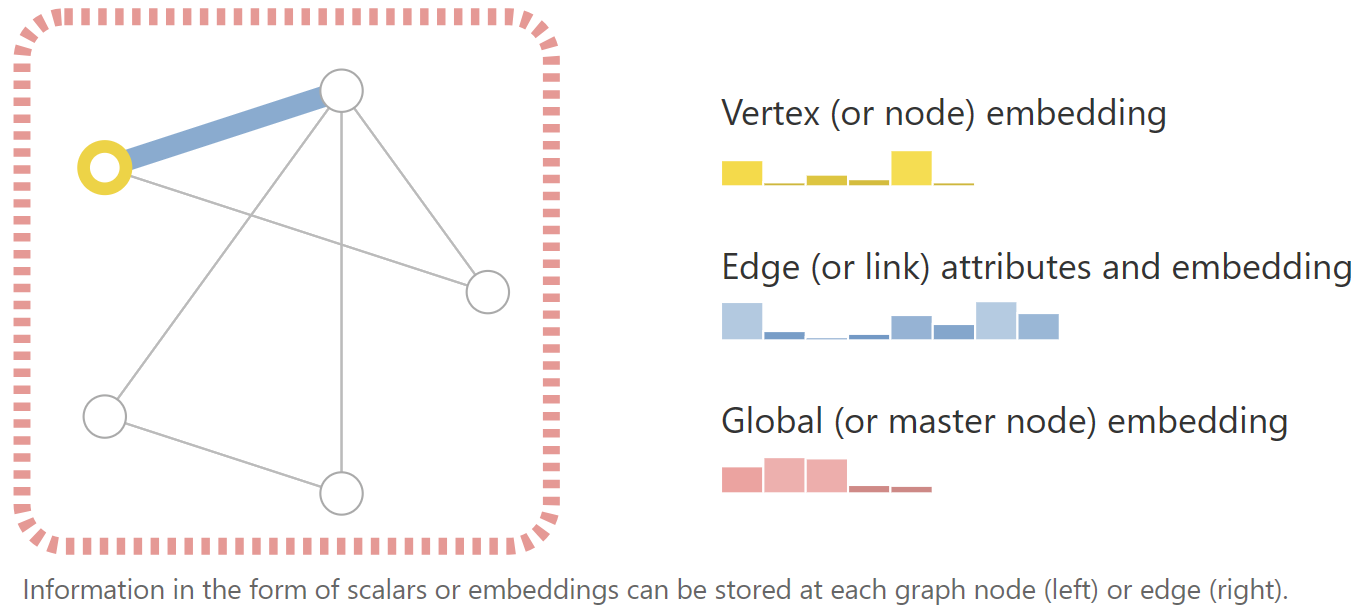
\includegraphics[width=\textwidth]{graph.png}
    \end{figure}
    图的三种元素都可以包含嵌入向量, 这里嵌入是一维的, 可视化呈现.
\end{frame}

\section{哪里有图结构?}

\begin{frame}{图像}
    \begin{figure}
        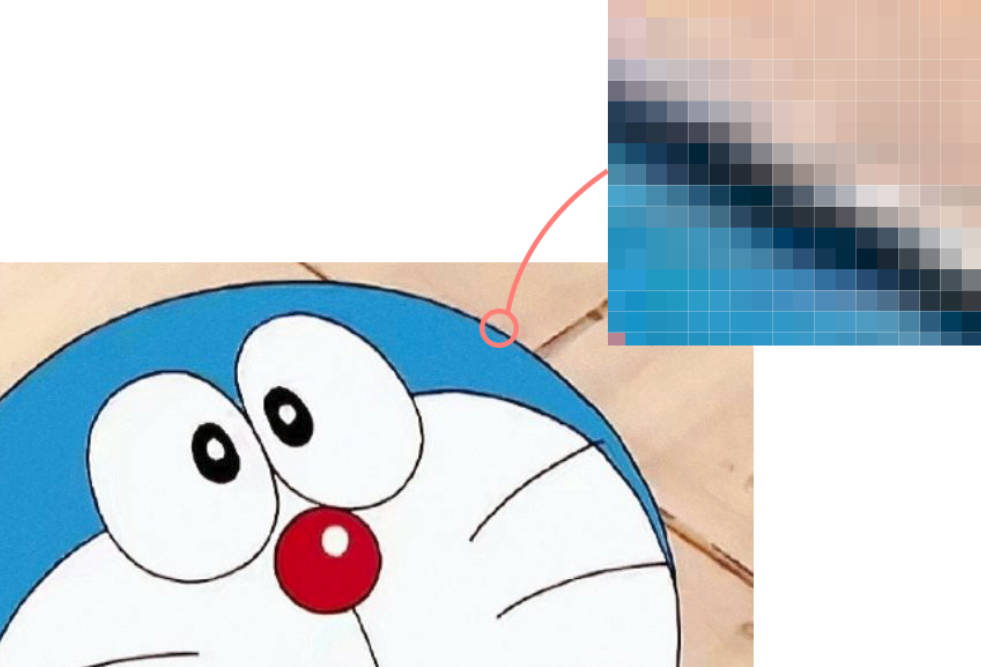
\includegraphics[width=0.5\textwidth]{图片像素.jpg}
        \caption{图片是由许多像素点构成的, 每个像素点有一个或多个数值, 如灰度值或者RGB值. }
    \end{figure}
\end{frame}

\begin{frame}{从图像到图}
    \begin{figure}
        \includegraphics[width=\textwidth]{图1.jpg}
        \caption{左边是图像, 中间是邻接矩阵, 右边是图. }
    \end{figure}
    图像也可以表示为图, 一个5*5的图像可以表示为邻接矩阵和图的形式. 这里三种不同的表现方法是同一个信息的不同表示方法.
\end{frame}

\begin{frame}{句子表示为图}
    \begin{figure}
        \includegraphics[width=\textwidth]{图2.jpg}
        \caption{语句表现为图的形式. }
    \end{figure}
    这里邻接矩阵去掉了对角连接和下三角表示. 另外, 语句在机器学习中通常不会用图表示, 而是通过编码并映射到嵌入向量.
\end{frame}

\begin{frame}{分子结构图}
    \begin{figure}
        \includegraphics[width=\textwidth]{图3.jpg}
        \caption{分子结构表现为图. }
    \end{figure}
    相比于前面的图, 分子图更具有异质性.
\end{frame}

\begin{frame}{人物关系图}
    \begin{figure}
        \includegraphics[width=\textwidth]{图4.jpg}
        \caption{人物关系建模为图. }
    \end{figure}
    话剧奥赛罗中的人物关系可以建模为图, 节点表现为角色, 边建模为人物间联系.
\end{frame}

\begin{frame}{论文引用关系图}
    \begin{figure}
        \includegraphics[width=0.5\textwidth]{图5.jpg}
        \caption{文章引用表示为图}
    \end{figure}
\end{frame}

\section{图任务}

\begin{frame}{图分类任务}
    \begin{figure}
        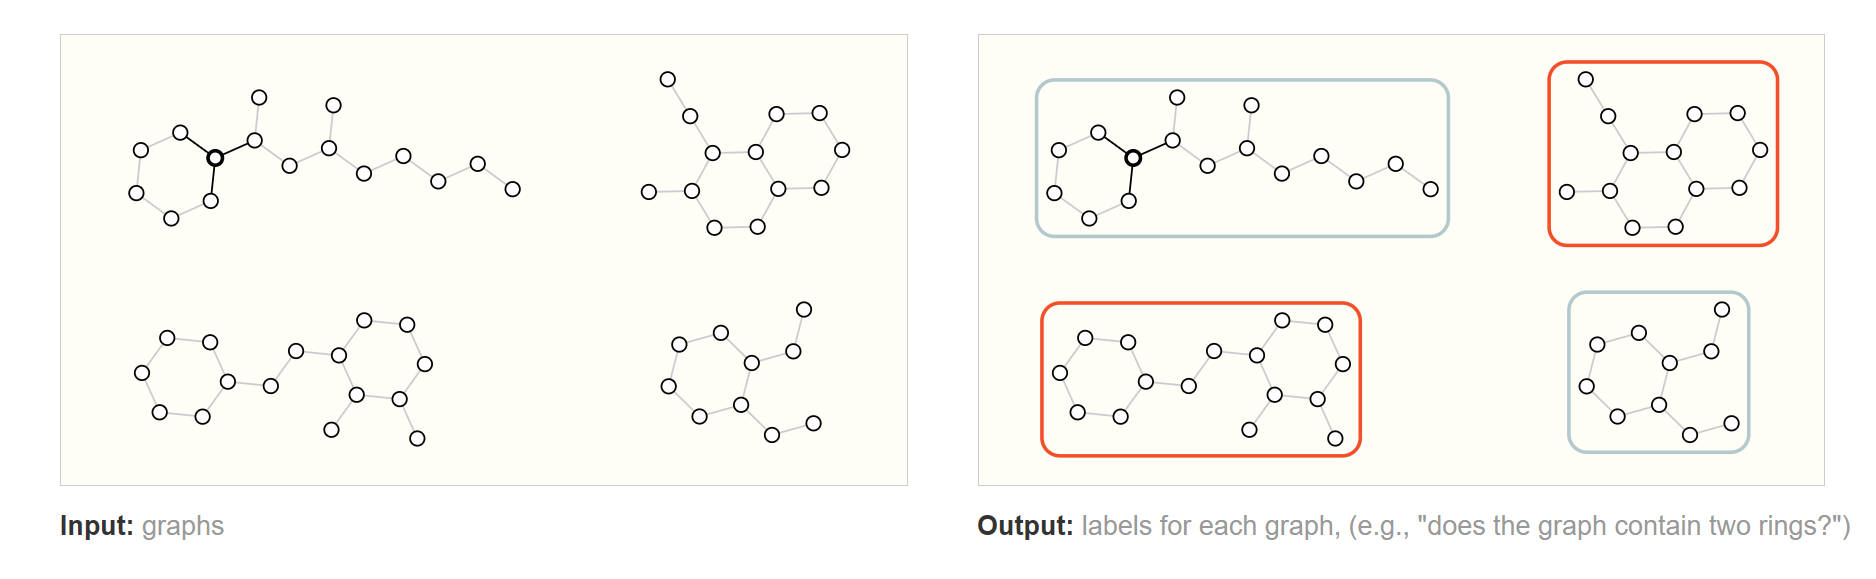
\includegraphics[width=\textwidth]{全局分类.jpg}
        \caption{识别哪些分子有两个苯环}
    \end{figure}
    输入多个分子的图信息, 输出各个图的类别.
\end{frame}

\begin{frame}{点分类任务}
    \begin{figure}
        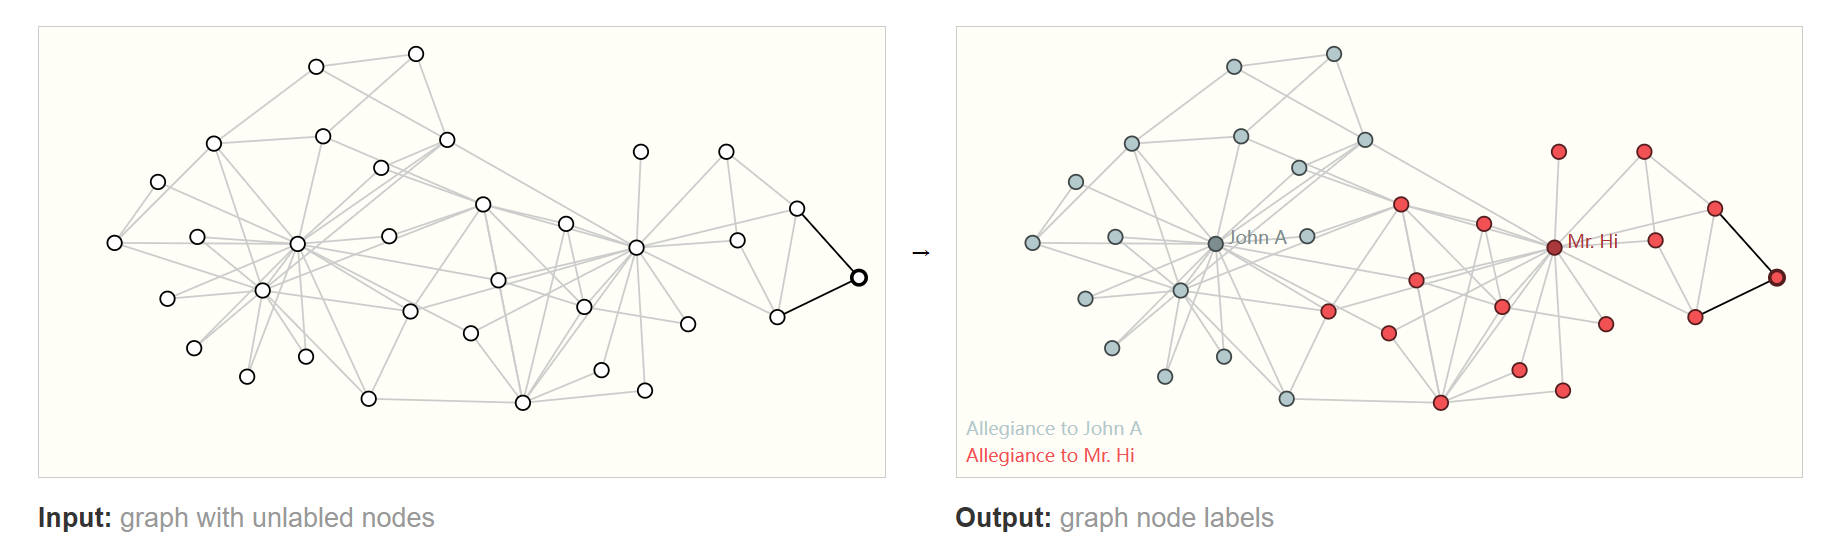
\includegraphics[width=\textwidth]{点分类.jpg}
        \caption{识别那些人支持John H, 哪些人支持Hi. }
    \end{figure}
    输入一个图, 输出各个点的类别, 这里是二分类.
\end{frame}

\begin{frame}{边分类任务}
    \begin{figure}
        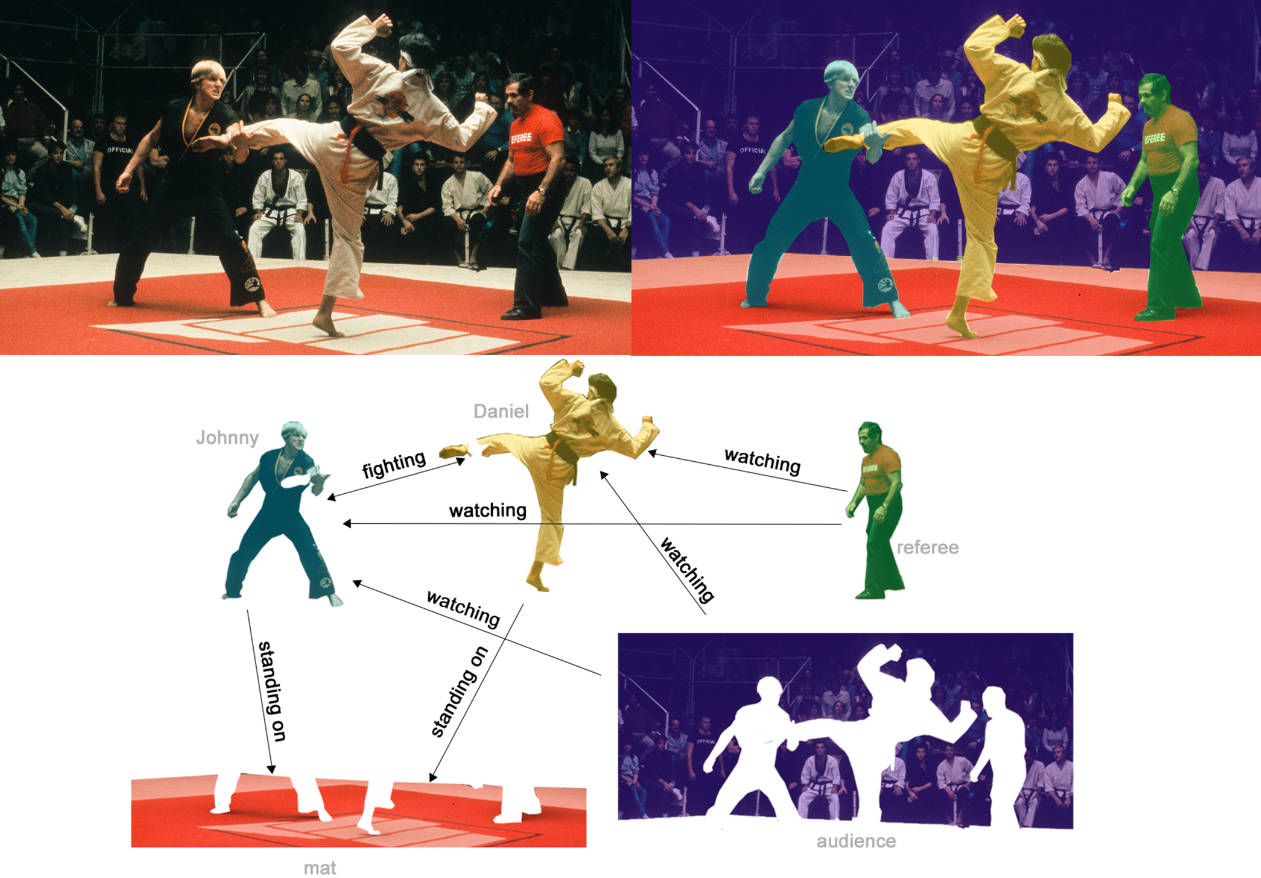
\includegraphics[width=0.7\textwidth]{边分类.jpg}
        \caption{先对图片做分割, 然后把被分割的部分作为节点, 识别各个节点之间的关系. 对局者站在垫子上, 对局者相互对抗, 裁判和观众观看对抗. }
    \end{figure}
\end{frame}

\begin{frame}{边分类任务}
    \begin{figure}
        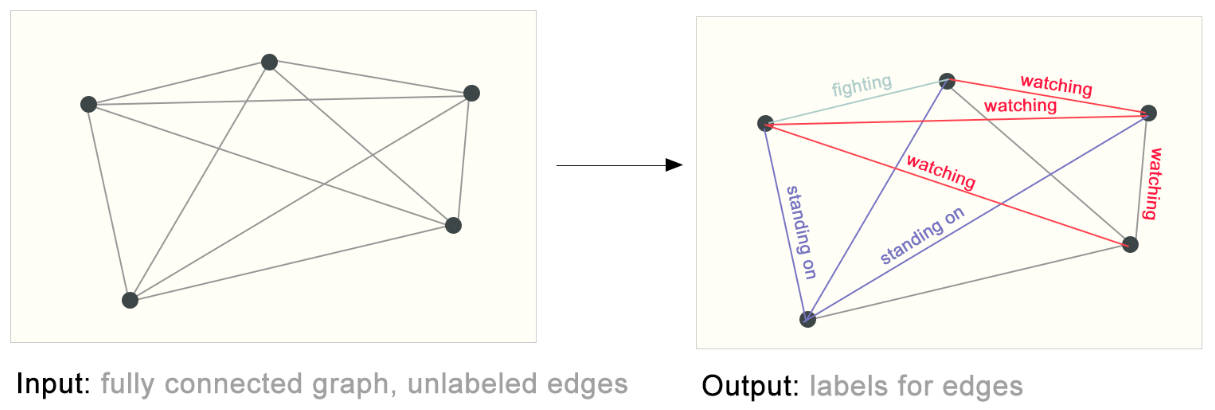
\includegraphics[width=\textwidth]{边分类2.jpg}
        \caption{图 9 简化图. }
    \end{figure}
\end{frame}

\section{图的构建}

\begin{frame}{邻接矩阵不足以表示图信息}
    \begin{figure}
        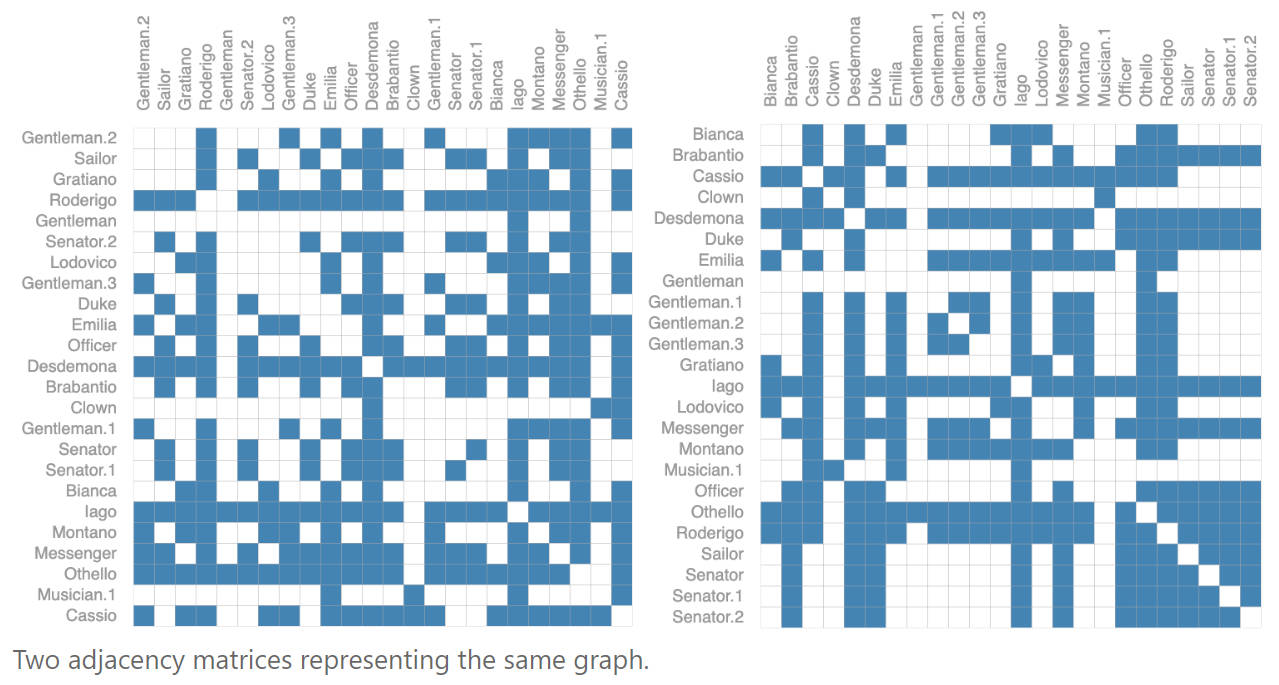
\includegraphics[width=0.9\textwidth]{邻接矩阵.jpg}
        \caption{邻接矩阵经过初等变换, 即行变换或者列变换, 其含义并没有改变, 但是矩阵特征发生很大改变. }
    \end{figure}
\end{frame}

\begin{frame}{邻接矩阵不足以表示图信息}
    \begin{figure}
        \includegraphics[width=0.9\textwidth]{图7.jpg}
        \caption{简单例子}
    \end{figure}
\end{frame}

\begin{frame}{图嵌入}
    下面的图片展示了图如何构建为嵌入向量, 需要注意的是, 在邻接表(edge\_index)中, 哪两个节点有连接是按列表示的, 也同时按照顺序定义了方向.
    \begin{figure}
        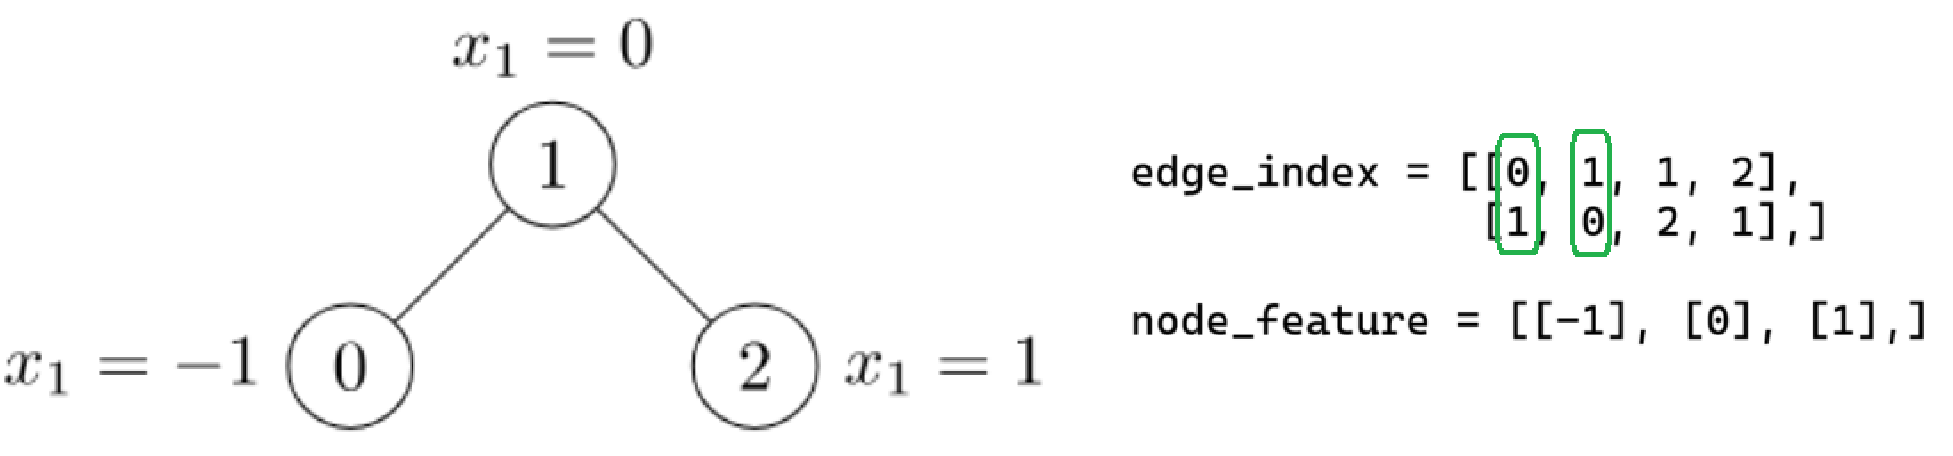
\includegraphics[width=\textwidth]{graph_sample.png}
        \caption{邻接矩阵无法用于学习, 但是图可以转化为嵌入向量形式以学习. 通过edge\_index、node\_feature等若干嵌入向量可以准确表示图信息. }\label{图嵌入}
    \end{figure}
\end{frame}

\begin{frame}{图嵌入}
    \begin{itemize}[<+-| alert@+>]
        \item 以节点举例, 图 \ref{图嵌入} 中一个节点的属性可以表示为-1,0,-1三个数字, 也可以表示为任意维度的张量, 其他元素同理.
        \item 如果一个节点表示一个学生, 它的节点属性可以是包含多个信息的向量, 比如[性别、班级、学校].
        \item 如果要对节点分类, 可以给出节点标签;如果是对图分类, 可以给出图标签, 此时节点标签就不是必要的, 比较重要的是节点特征和邻接表:节点特征是图的基本信息, 邻接表引定义图结构.
        \item 这里的邻接表可以表示为其他不同的形式, 以使用的图网络的包的要求为准.
    \end{itemize}
\end{frame}

\section{图神经网络}

\subsection{处理图结构的基础方法}

\begin{frame}{分开处理每个嵌入向量}
    \begin{figure}
        \centering
        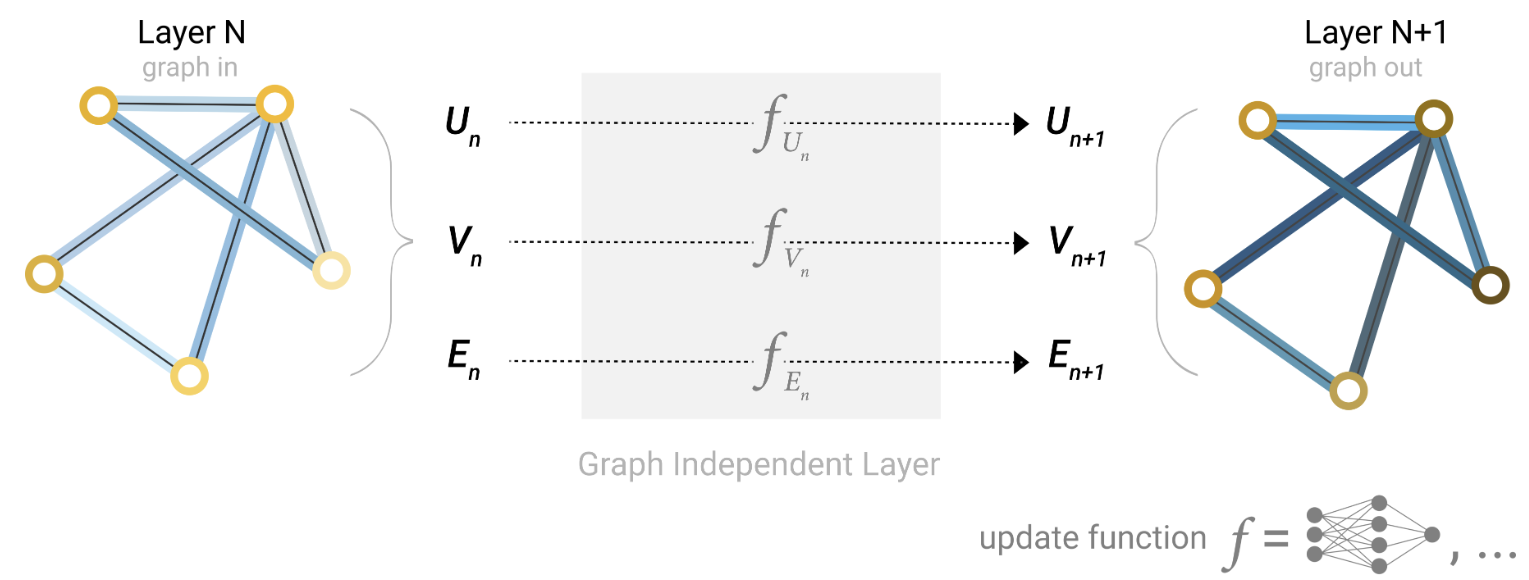
\includegraphics[width=0.9\textwidth]{简易GNN.png}
        \caption{简易GNN. 前面我们已经把图转化成包含点信息、边信息、全局信息的嵌入形式, 因此我们可以分别构建三个神经网络去学习它们各自的特征. 另外, 这里图神经网络没有改变节点直接的连接性, 因此经过处理前后的邻接矩阵也不会变化. }
    \end{figure}
\end{frame}

\begin{frame}{基础点分类}
    \begin{figure}
        \centering
        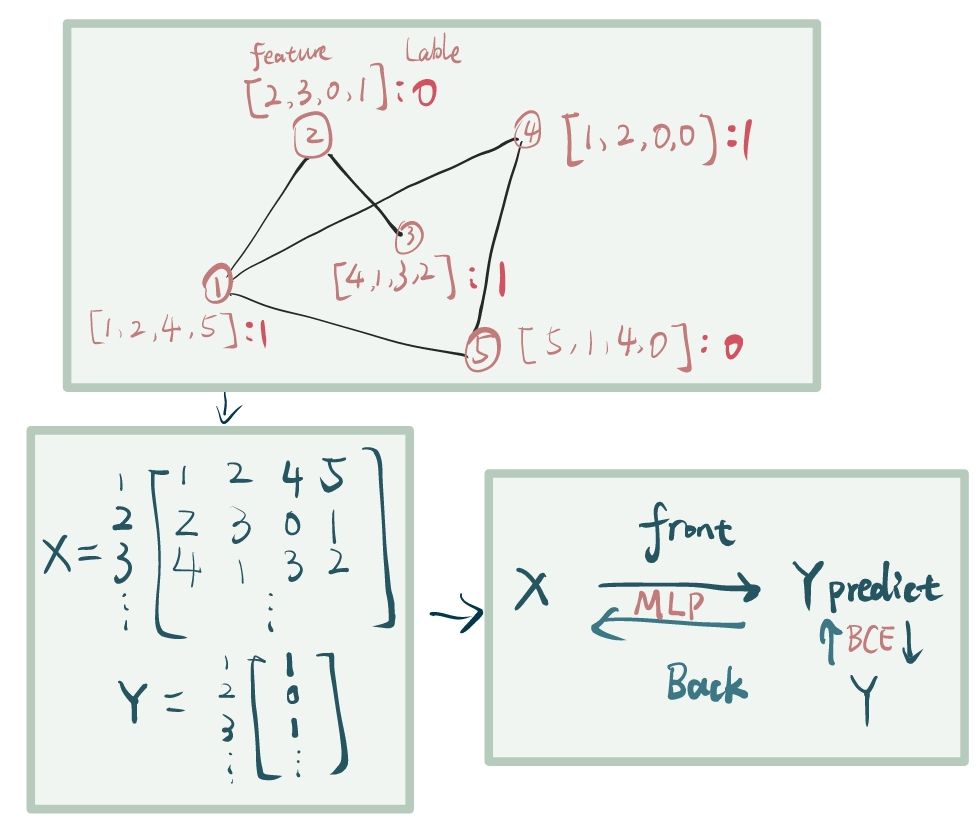
\includegraphics[width=0.6\textwidth]{点分类例子.png}
        \caption{基础点分类图解. 把点特征整理为一个矩阵, 点标签整理为列向量, 发现与普通机器学习并无区别. 边分类和图分类同理. }
    \end{figure}
\end{frame}

\subsection{基础图神经网络}

\begin{frame}{信息传递}
    \textbf{信息传递是图神经网络的关键要素.}
    \begin{figure}
        \centering
        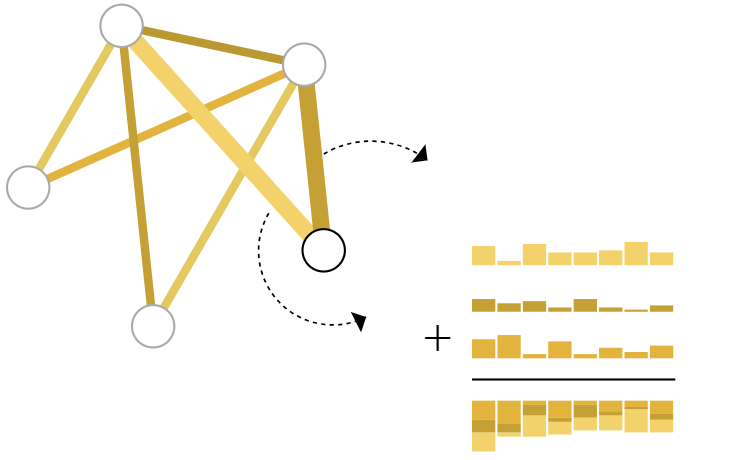
\includegraphics[width=0.5\textwidth]{信息传递.png}
        \caption{信息传递机制. 信息传递也叫聚合. 一个节点可以从与其连接的边或者节点聚合信息. 边也可以聚合节点的信息. 边嵌入和点嵌入至少要有一个. 聚合操作一般是指池化. 聚合之后同样可以通过MLP学习.}
    \end{figure}
    问题:1. 池化会不会损失太多信息?
\end{frame}

\begin{frame}{节点信息聚合到全局}
    \begin{figure}
        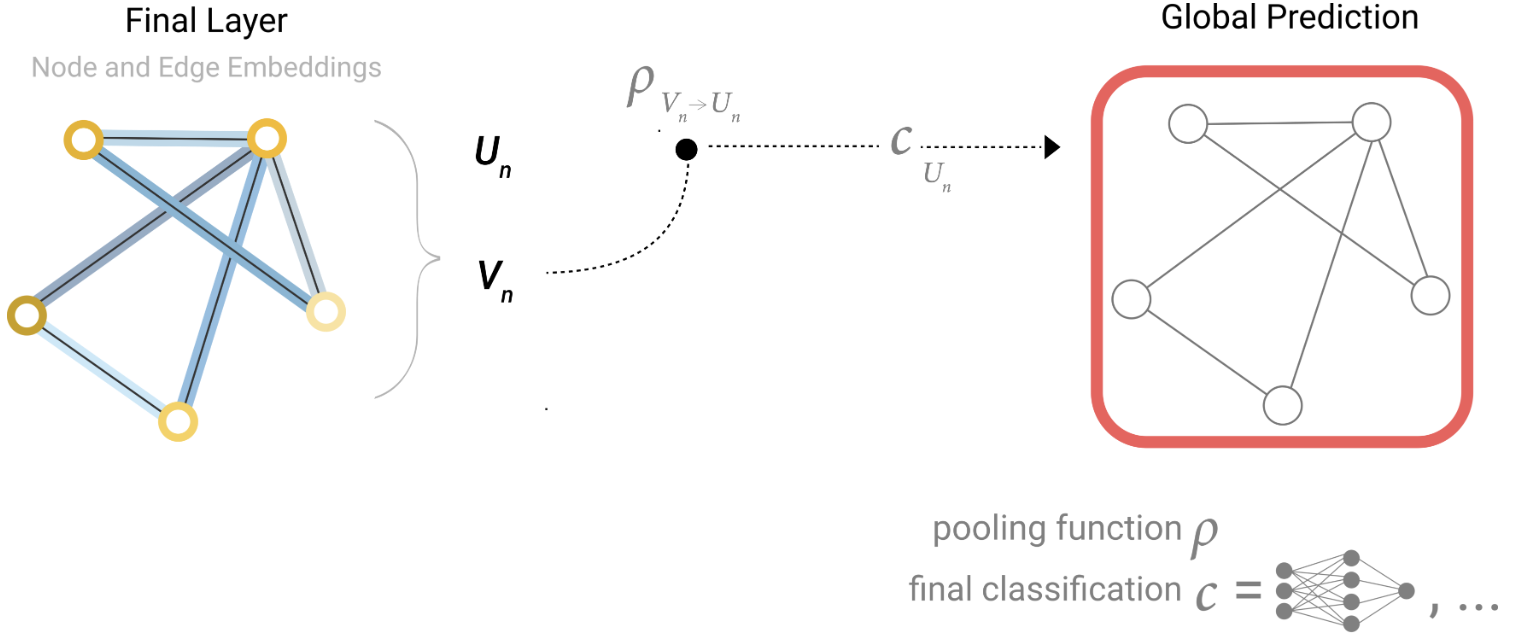
\includegraphics[width=\textwidth]{节点预测全局.png}
        \caption{节点预测全局. 对全局节点做池化聚合到全局嵌入, 可以实现全局信息聚合. 同理还可以聚合边的信息到全局.}
    \end{figure}
\end{frame}

\begin{frame}{比较复杂的聚合}
    \begin{figure}
        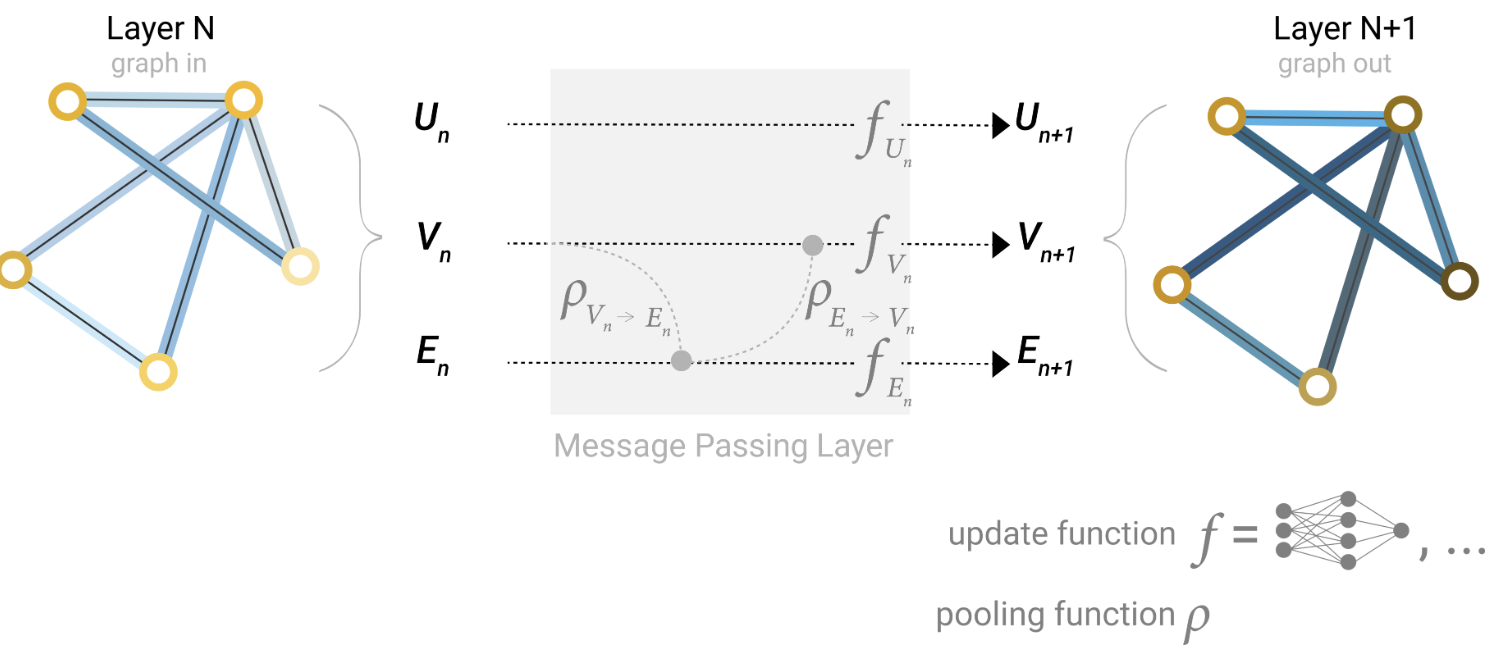
\includegraphics[width=0.9\textwidth]{节点到边到节点聚合.png}
        \caption{节点-边-节点聚合.}
    \end{figure}
\end{frame}

\begin{frame}{比较复杂的聚合}
    \begin{figure}
        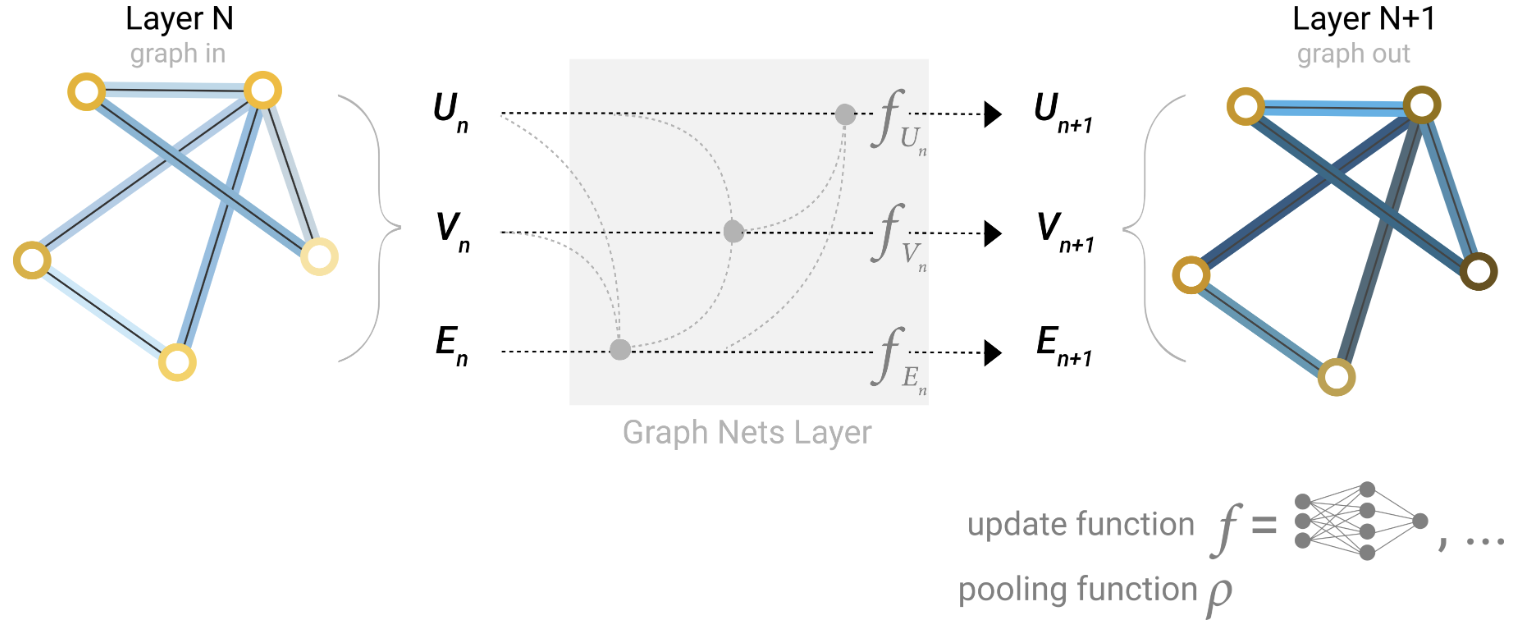
\includegraphics[width=\textwidth]{节点边全局聚合.png}
        \caption{节点-边-全局混合聚合.}
    \end{figure}
\end{frame}

\begin{frame}
    \begin{itemize}
        \item 池化聚合是最简单的方法之一, 图卷积方法是现在的主流聚合方案, 在此基础上很容易加入注意力机制.
        \item 值得注意的是图卷积和图像卷积在操作上几乎没有相同点.
        \item 创新聚合方法是一种主要的改进方向.
    \end{itemize}
\end{frame}

\begin{frame}
    \begin{figure}
        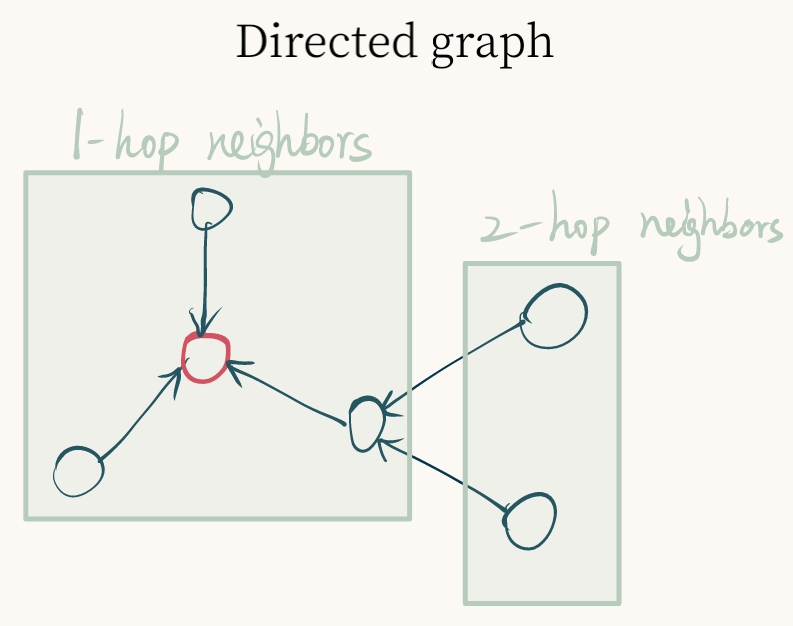
\includegraphics[width=0.5\textwidth]{有向图.png}
        \caption{一种有向图. 这表示边是单向的, 消息传递只能按照边方向进行. 其中红色节点包括1-hop邻居和2-hop邻居.}
    \end{figure}
    \begin{block}{Note}
        无向图是指边双向连接而不是无方向连接.
    \end{block}
\end{frame}

\begin{frame}
    \begin{figure}
        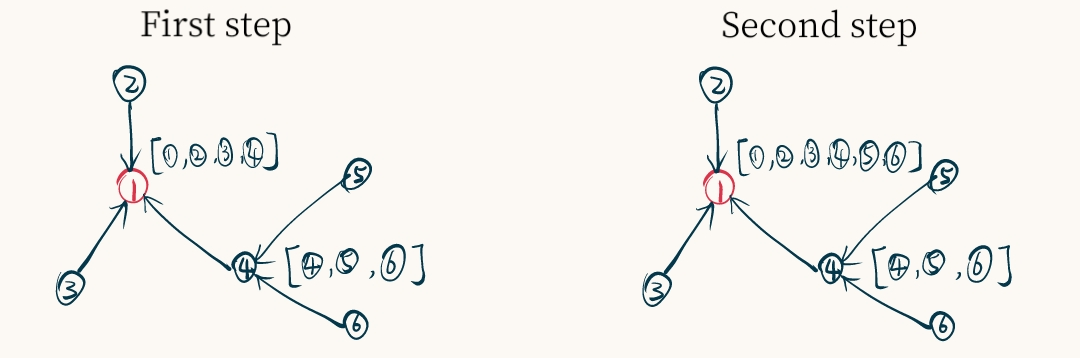
\includegraphics[width=0.9\textwidth]{两步消息传递.png}
        \caption{对于红色节点, 通过两次信息传递就可以获得全局信息.}
    \end{figure}
    每一次信息传递都伴随一次神经网络处理, 因此这里的step可以看作神经网络中的epoch, 两步消息传递也就是两个epoch. 这里仅构建了有向图, 对于无向图来说, 每个节点每一步都在聚合邻居信息.
\end{frame}

\subsection{图卷积}

\begin{frame}{方法一}
    \small
    \vspace{-1cm}
    \begin{multicols}{2}
        \[
            A =
            \begin{bmatrix}
                0 & 1 & 0 & 1 \\
                1 & 0 & 1 & 1 \\
                0 & 1 & 0 & 0 \\
                1 & 1 & 0 & 0 \\
            \end{bmatrix}
        \]

        \[
            H =
            \begin{bmatrix}
                h_{11} & \ldots & \ldots & \ldots \\
                h_{21} & \ldots & \ldots & \ldots \\
                h_{31} & \ldots & \ldots & \ldots \\
                h_{41} & \ldots & \ldots & \ldots \\
            \end{bmatrix}
        \]
    \end{multicols}

    这里随机给出一个邻接矩阵 \(A\) 和其度矩阵 \(D\),最简单的聚合公式是:
    \[ H^{(t+1)} = \sigma(AH^{(t)}W^{(t)}) \]
    \(H\) 是特征矩阵,包含所有节点的特征,所有上标都表示更新步,\(\sigma\) 是非线性激活函数,\(A\) 是邻接矩阵,之前说过图神经网络不改变连接性,因此 \(A\) 是不变的,\(W\) 是可训练的权重矩阵,等于神经网络的线性映射.
\end{frame}

\begin{frame}{方法一}
    \begin{figure}
        \centering
        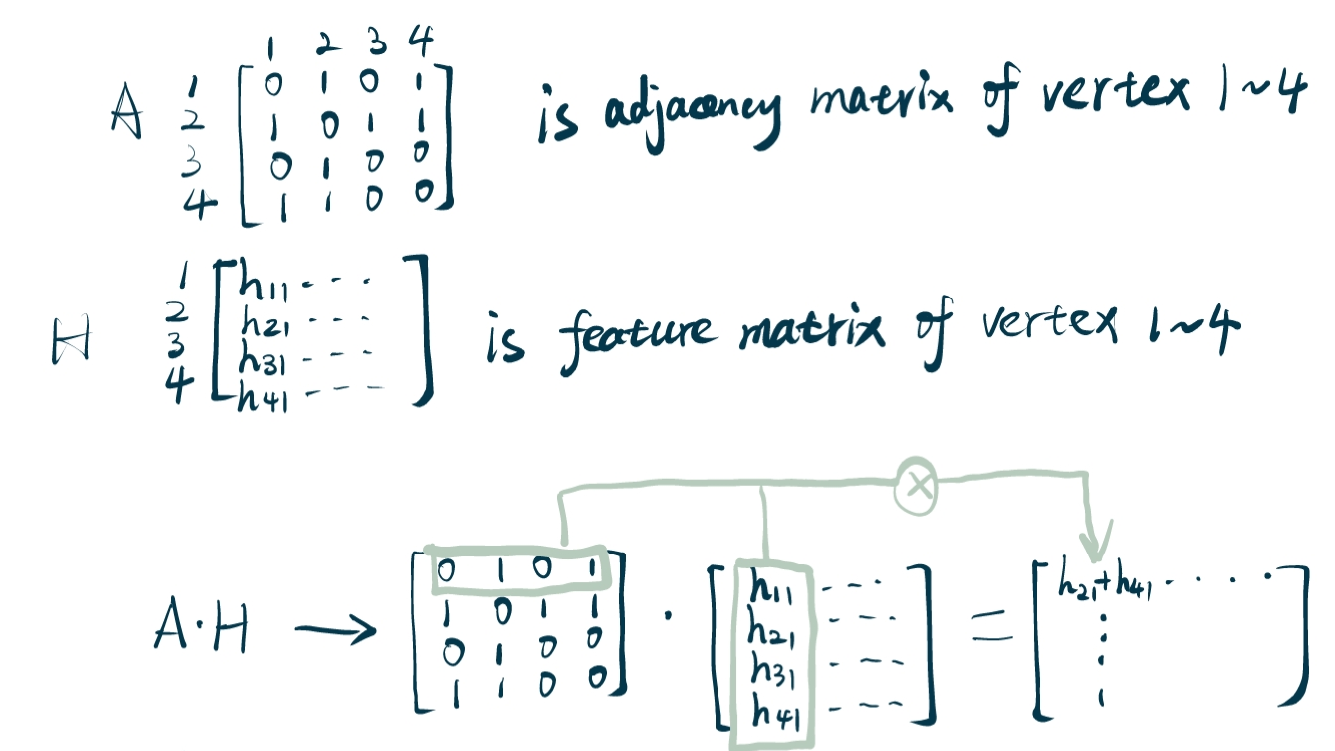
\includegraphics[width=0.8\textwidth]{聚合1.png}
        \caption{$AH$运算使得$h_{11}$变为$h_{21}+h_{41}$, 因为$V_{11}$与节点$V_{21}, V_{41}$相邻.}
    \end{figure}
    但是这样运算显然丢失了$V_{11}$自己的信息. 其他节点同理.
\end{frame}

\begin{frame}{方法二}\footnotesize
    \begin{multicols}{3}
        \[
            A =
            \begin{bmatrix}
                0 & 1 & 0 & 1 \\
                1 & 0 & 1 & 1 \\
                0 & 1 & 0 & 0 \\
                1 & 1 & 0 & 0 \\
            \end{bmatrix}
        \]

        \[
            D =
            \begin{bmatrix}
                2 & 0 & 0 & 0 \\
                0 & 3 & 0 & 0 \\
                0 & 0 & 1 & 0 \\
                0 & 0 & 0 & 2 \\
            \end{bmatrix}
        \]

        \[
            L =
            \begin{bmatrix}
                2  & -1 & 0  & -1 \\
                -1 & 3  & -1 & -1 \\
                0  & -1 & 1  & 0  \\
                -1 & -1 & 0  & 2  \\
            \end{bmatrix}
        \]
    \end{multicols}
    引入度矩阵$D$, 表现为一个节点有多少个入度, 构建拉普拉斯矩阵(Combinatorial Laplacian) $L$:
    $$L = D - A$$
    图卷积更新公式:
    $$ H^{(t+1)} = \sigma(LH^{(t)}W^{(t)}) $$
    这样在运算时就考虑了节点自身的信息. 但有些节点的度可能非常大, 从而显著影响分类效果, 所以方法三对$L$矩阵做了标准化.
\end{frame}

\begin{frame}{方法三: 最常用的图卷积方法}\footnotesize
    \vspace{-0.5cm}
    \begin{multicols}{2}
        \[
            D =
            \begin{bmatrix}
                2 & 0 & 0 & 0 \\
                0 & 3 & 0 & 0 \\
                0 & 0 & 1 & 0 \\
                0 & 0 & 0 & 2 \\
            \end{bmatrix}
        \]
        \[
            A =
            \begin{bmatrix}
                0 & 1 & 0 & 1 \\
                1 & 0 & 1 & 1 \\
                0 & 1 & 0 & 0 \\
                1 & 1 & 0 & 0 \\
            \end{bmatrix}
        \]
        \[
            D^{-\frac{1}{2}} =
            \begin{bmatrix}
                \sqrt{2}^{-1} & 0             & 0 & 0             \\
                0             & \sqrt{3}^{-1} & 0 & 0             \\
                0             & 0             & 1 & 0             \\
                0             & 0             & 0 & \sqrt{2}^{-1}
            \end{bmatrix}
        \]
        \[
            \tilde{L} = \begin{bmatrix}
                1                   & -\frac{1}{\sqrt{6}} & 0                   & -\frac{1}{2}        \\
                -\frac{1}{\sqrt{6}} & 1                   & -\frac{1}{\sqrt{3}} & -\frac{1}{\sqrt{6}} \\
                0                   & -\frac{1}{\sqrt{3}} & 1                   & 0                   \\
                -\frac{1}{2}        & -\frac{1}{\sqrt{6}} & 0                   & 1
            \end{bmatrix}
        \]

    \end{multicols}
    前面已经介绍了$L$的公式: $L=D-A$, 可以通过度矩阵标准化A, 然后给出$\tilde{L}$, 这里给出标准化公式:
    $$ \tilde{L} = D^{-\frac{1}{2}}(D-A)D^{-\frac{1}{2}} = I - D^{-\frac{1}{2}}AD^{-\frac{1}{2}} $$
    通过标准化, 将度和邻接表示进行放缩, 其中度被放缩到1, 从而避免了了数值太大影响分类效果.\\
\end{frame}

\begin{frame}{方法三: 最常用的图卷积方法}
    最后,给出最常见的图卷积表达式:
    $$H^{(t+1)} = \sigma(\tilde{L}H^{(t)}W^{(t)})$$
    在图卷积中,由于每次卷积都是在聚合邻居的信息,因此每一对邻居节点都可以依据自身的特征给对方分配一个注意力分数,这就是图卷积注意力方法。
    \newline

    现在你可以调包了:)
    \newline

    PyTorch Geometric是图网络常用的包之一
    \url{https://pytorch-geometric.readthedocs.io/en/latest/index.html}
\end{frame}

\section{总结}

\begin{frame}
    \begin{itemize}
        \item 图需要转化为嵌入向量才能被处理;
        \item 图非常擅长描述具有拓扑结构的数据;
        \item 图神经网络的特点在于信息传递。
    \end{itemize}
\end{frame}

\section{参考文献}

\begin{frame} %[allowframebreaks]
    \bibliography{ref}
    \bibliographystyle{plain}
    % 如果参考文献太多的话, 可以像下面这样调整字体:
    % \tiny\bibliographystyle{alpha}
\end{frame}

\begin{frame}
    \begin{center}
        {\Huge\calligra Thanks!}
    \end{center}
\end{frame}

\end{document}